\subsubsection{Panel frontal}


El panel frontal del SAL/T sigue el diseño de la figura \ref{fig:panel_frontal} utilizando una placa secundaria donde se colocan directamente los LEDs (\textit{Light-Emitting Diode}), el display de velocidad, el botón seleccionador de perfil intermitente y un buzzer sonoro. \\ 

El panel frontal cuenta con cuatro LEDs verdes utilizados para indicar el estado de la alimentación, el modo aislado limitado, el modo aislado total y el perfil intermitente seleccionados; diez LEDs RGB (\textit{Red Green Blue}) para indicar el estado de los SIS, de las señales de CT y FE, la presencia de un comando remoto activo, el estado del receptor GPS y un indicador de la zona de circulación actual de la formación; un botón para seleccionar el perfil intermitente a utilizar; el display de velocidad de cuatro dígitos 7 segmentos y la llave interruptora que queda por fuera de la placa secundaria. \\ 

Para controlar todos estos LEDs y el display de velocidad, se utilizó el controlador LED AS1115-BSST de ams OSRAM \cite{AS1115-BSST}. Este permite controlar hasta sesenta y cuatro LEDs u ocho dígitos de un display 7 segmentos reduciendo la cantidad de pines necesarios a utilizar del MCU ya que se conecta por protocolo I2C utilizando solamente dos cables. Este controlador permite setear la corriente de cada LED utilizando una resistencia externa; en este caso, siguiendo los valores normalizados y recomendados por la hoja de datos del controlador, se colocó una resistencia de 22 k$\Omega$ para obtener una corriente de 10 mA. El controlador también trae entradas para la detección de hasta dieciséis teclas en una matriz de teclas, pero esa funcionalidad no se utiliza en esta aplicación. \\



El AS1115-BSST utiliza un método de multiplexado en el cual cada grupo de LEDs o segmentos es controlado secuencialmente, encendiéndolos en rápida sucesión. Esto reduce la cantidad de pines necesarios para el control, ya que todos los LEDs no están encendidos simultáneamente, pero debido a la alta velocidad de escaneo, se perciben como si estuvieran encendidos de forma continua. Además, a través de la interfaz I2C, se envían comandos para controlar el brillo, encendido y apagado de los LEDs o segmentos, y se pueden ajustar los valores de corriente para mejorar la eficiencia energética.\\




En la figura \ref{fig:led_driver} se observa una aplicación típica de este controlador; para el SAL/T, se utilizó una alimentación de 5 V, un Rset = 22 k$\Omega$, la comunicación con el MCU solo con las líneas de SDA y SCL de I2C trabajando a 100 kHz sin el pin de interrupción, no se utilizaron las entradas de detección de teclas, y se conectó al display de cuatro dígitos 7 segmentos y a los LEDs mencionados previamente. \\

\begin{figure}[H]
    \centering
    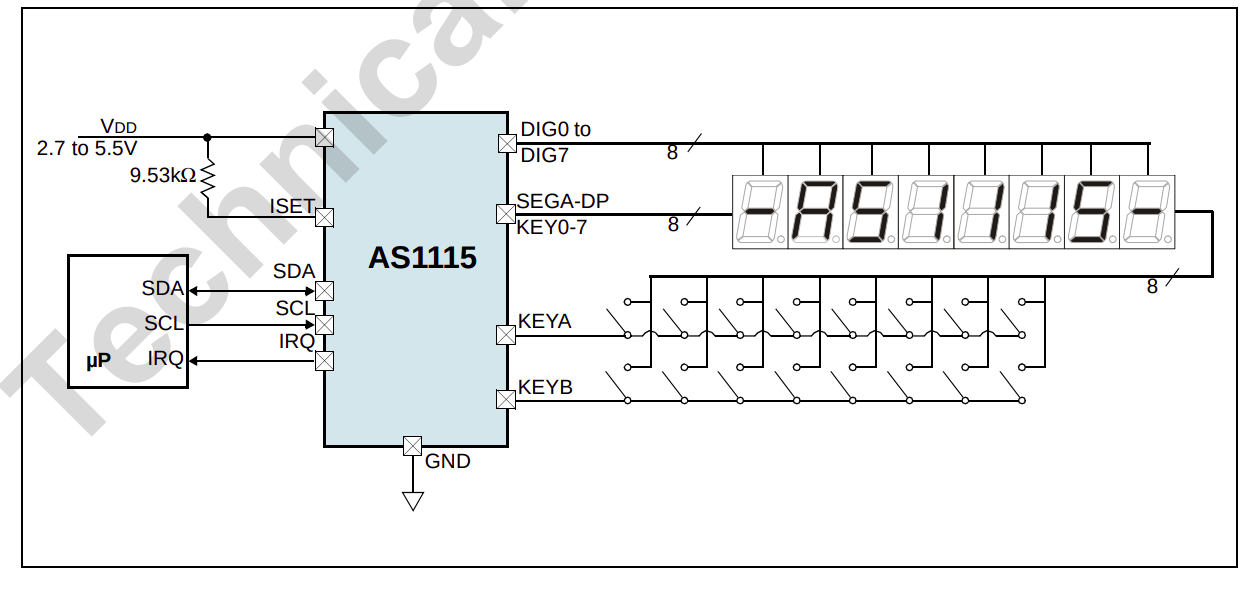
\includegraphics[width = \linewidth]{img/led_driver.png}
    \caption{Aplicación típica de un controlador AS1115-BSST}
    \label{fig:led_driver}
\end{figure}    




Para los LEDs RGB utilizados se seleccionó el modelo WP154A4SEJ3VBDZGW/CA de Kingbright \cite{WP154A4SEJ3VBDZGW/CA} diseñado para aplicaciones que requieren indicación de estado multicolor. Ofrece alta luminosidad y bajo consumo de energía, con un encapsulado transparente de 5 mm, lo que lo hace ideal para proyectos que requieren señalización visual con múltiples colores en un solo componente. Trabajan con una corriente máxima de 20 mA por color, y tienen una caída de tensión e intensidad luminosa para cada color de: 

\begin{itemize}
    \item Rojo: 2 V - 300 mcd
    \item Verde: 3,3 V - 600 mcd
    \item Azul: 3,3 V - 500 mcd
\end{itemize}

Estos LEDs se montan \textit{through hole} y quedan sobresalientes a la placa para luego insertarlos dentro de un gabinete con agujeros para permitir la visualización de estos componentes. Tienen un encapsulado transparente y un lente de tipo redondo con un ángulo de visión de 30°.\\ 

Para los LEDs verdes se utilizó el modelo WP7113LZGCK de Kingbright \cite{WP7113LZGCK} que cuenta con características muy similares solo para el color verde del modelo RGB presentado. Las diferencias son que tiene una tensión Vf = 2,1 V, tolera una corriente máxima de 30 mA y su intensidad luminosa es un poco mayor, ya que puede llegar hasta 3000 mcd dependiendo de la corriente. \\ 

Para el display de velocidad se utilizó el modelo LTC-5723HR de Lite-On \cite{LTC-5723HR}; contiene cuatro dígitos con formato de 7 segmentos de color rojo en configuración cátodo común. Cada dígito tiene un tamaño de 8,1 x 14,2 mm. Funciona con una tensión directa de Vf = 2 V y corriente de hasta 20 mA por segmento. Es de montaje \textit{through-hole} lo que permite dejarlo visible por fuera de la placa con cierta separación. \\

En la figura \ref{fig:leds_model} se visualiza el display mencionado junto a un LED RGB y un LED verde utilizado para la implementación. 

\begin{figure}[H]
    \centering
    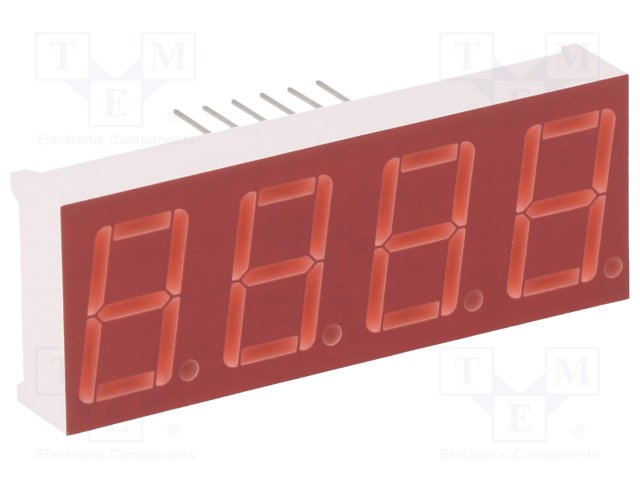
\includegraphics[width = 0.3 \linewidth]{img/display.jpg}
    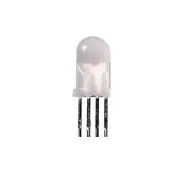
\includegraphics[width = 0.3 \linewidth]{img/led_rgb.png}
    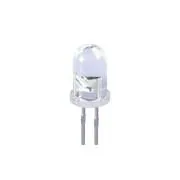
\includegraphics[width = 0.3 \linewidth]{img/led_g.png}
    \caption{Modelos utilizados para las indicaciones luminosas del panel frontal}
    \label{fig:leds_model}
\end{figure}    


Para el botón de selección del perfil intermitente se utilizó un interruptor con pulsador \textit{push switch} modelo de 1543-650-149 de Bourns \cite{1543-650-149} utilizando un circuito con una resistencia de \textit{pull-down} para forzar 0 V en la entrada del MCU cuando el interruptor está abierto y una resistencia para realizar un divisor resistivo de 5 V (alimentación de la placa) a 3,3 V (tensión de nivel alto de entrada digital del MCU). También se agregó una resistencia en serie de 100 Ohms. En la figura \ref{fig:chop_sel} se visualiza el circuito. 

\begin{figure}[H]
    \centering
    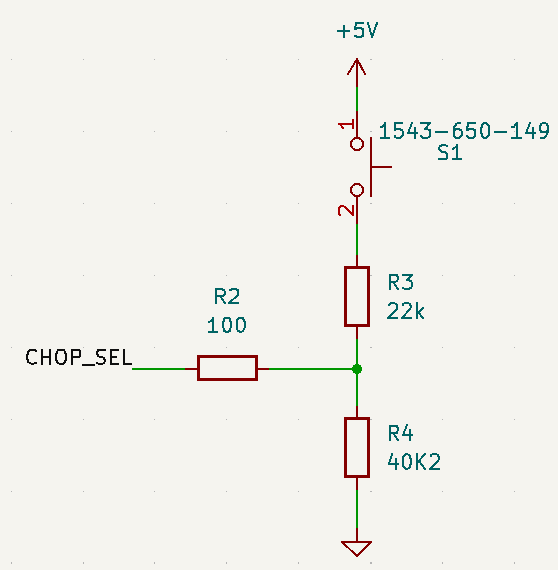
\includegraphics[width = 0.5 \linewidth]{img/chop_sel.png}
    \caption{Circuito del selector de perfil intermitente}
    \label{fig:chop_sel}
\end{figure}    


El panel frontal cuenta también con un buzzer sonoro que se activa de manera intermitente cuando se circula en modo aislado limitado y suena de manera continua cuando se exceden los límites de velocidad establecidos. Para el buzzer sonoro se utilizó el modelo CEM-1205-IC de SameSky \cite{CEM-1205-IC}. Este módulo cuenta con un oscilador interno que al energizarse con 5 VDC emite una señal sonora de 2400 Hz consumiendo 30 mA de corriente. Para el control del encendido de este módulo, se utilizó un transistor MOSFET canal P modelo NVTR0202PLT1G de onsemi \cite{NVTR0202PLT1G} conectado como se visualiza en la figura \ref{fig:buzzer_sch}. Cuando la señal de control BUZZER\_C está en estado bajo 0 V, el circuito permite la corriente y alimenta el buzzer sonoro; cuando la señal se coloca en un estado de alta impedancia, no circula corriente apagando el buzzer sonoro. También se colocó un capacitor de 10 $\mu$F para suavizar el sonido reduciendo los ruidos que puedan entrar por la línea de alimentación. 



\begin{figure}[H]
    \centering
    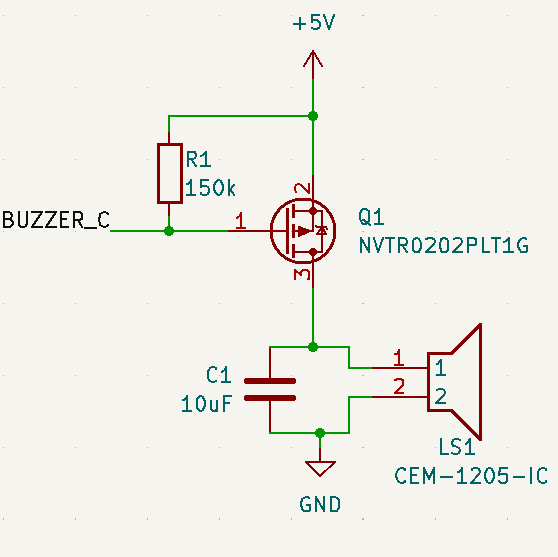
\includegraphics[width = 0.6 \linewidth]{img/buzzer.png}
    \caption{Circuito de activación del buzzer sonoro}
    \label{fig:buzzer_sch}
\end{figure}    


